\documentclass{classes/weekly_report}
\usepackage{comment}
\usepackage{url}
\usepackage{minted}

\title{
	真値と推定値の差を比較する機能の実装
}

\author{
	中島大河
}

\meetingdate{2026年6月31日} % ミーティングの日付を設定

% -------------------------ここから-------------------------

\begin{document}
\maketitle
\thispagestyle{preport}

% -------------------------ここまで触らない-------------------------

\section{目的}
真値と推定値の差を比較する機能を実装する。

\section{今週やったこと1:カメラシミュレートと誤差比較}
\Fig{fig:csv}に示すように単一画像から、カメラをシミュレートする動画と、その経路の真値をCSVとして吐き出すプログラムを作成した。

\begin{figure}[H]
    \centering
    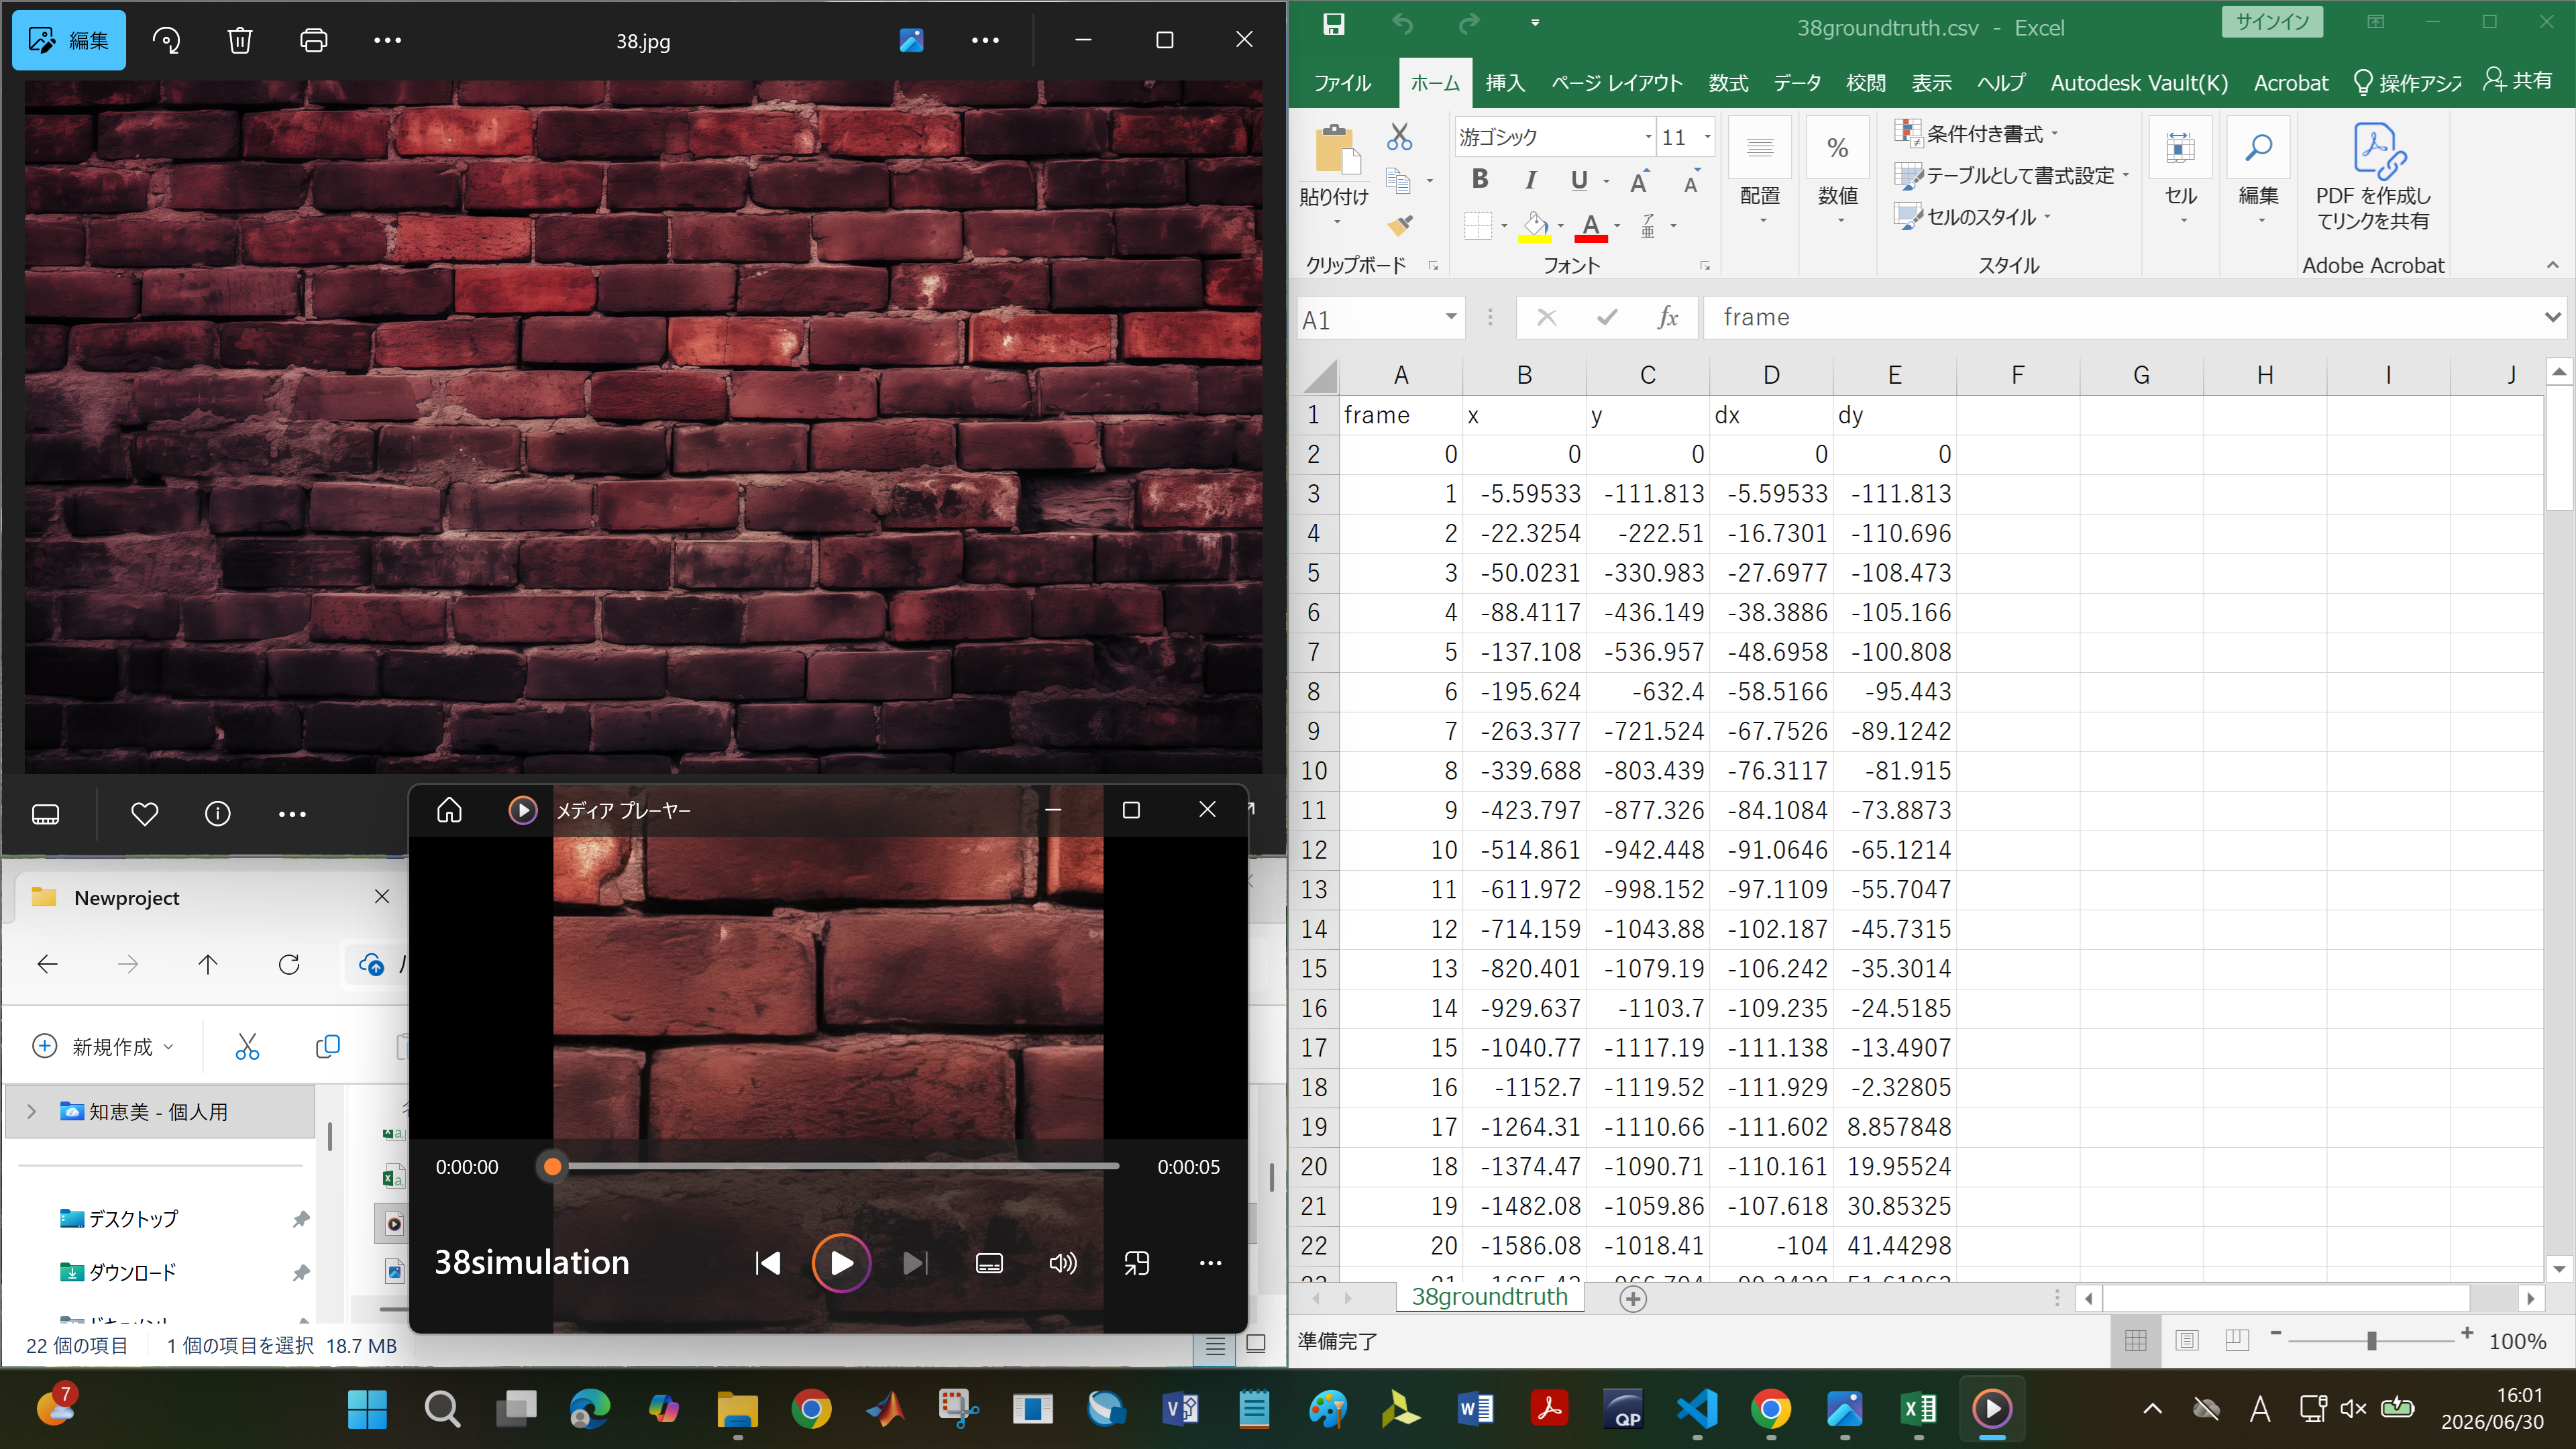
\includegraphics[width=\linewidth]{figures/csv.png}
    \caption{カメラシミュレート}
    \label{fig:csv}
\end{figure}

また、\Fig{fig:誤差比較}の様に真値と推定値の誤差やユークリッド距離を計算し、CSVとして吐き出す機能を実装した。


\begin{figure}[H]
    \centering
    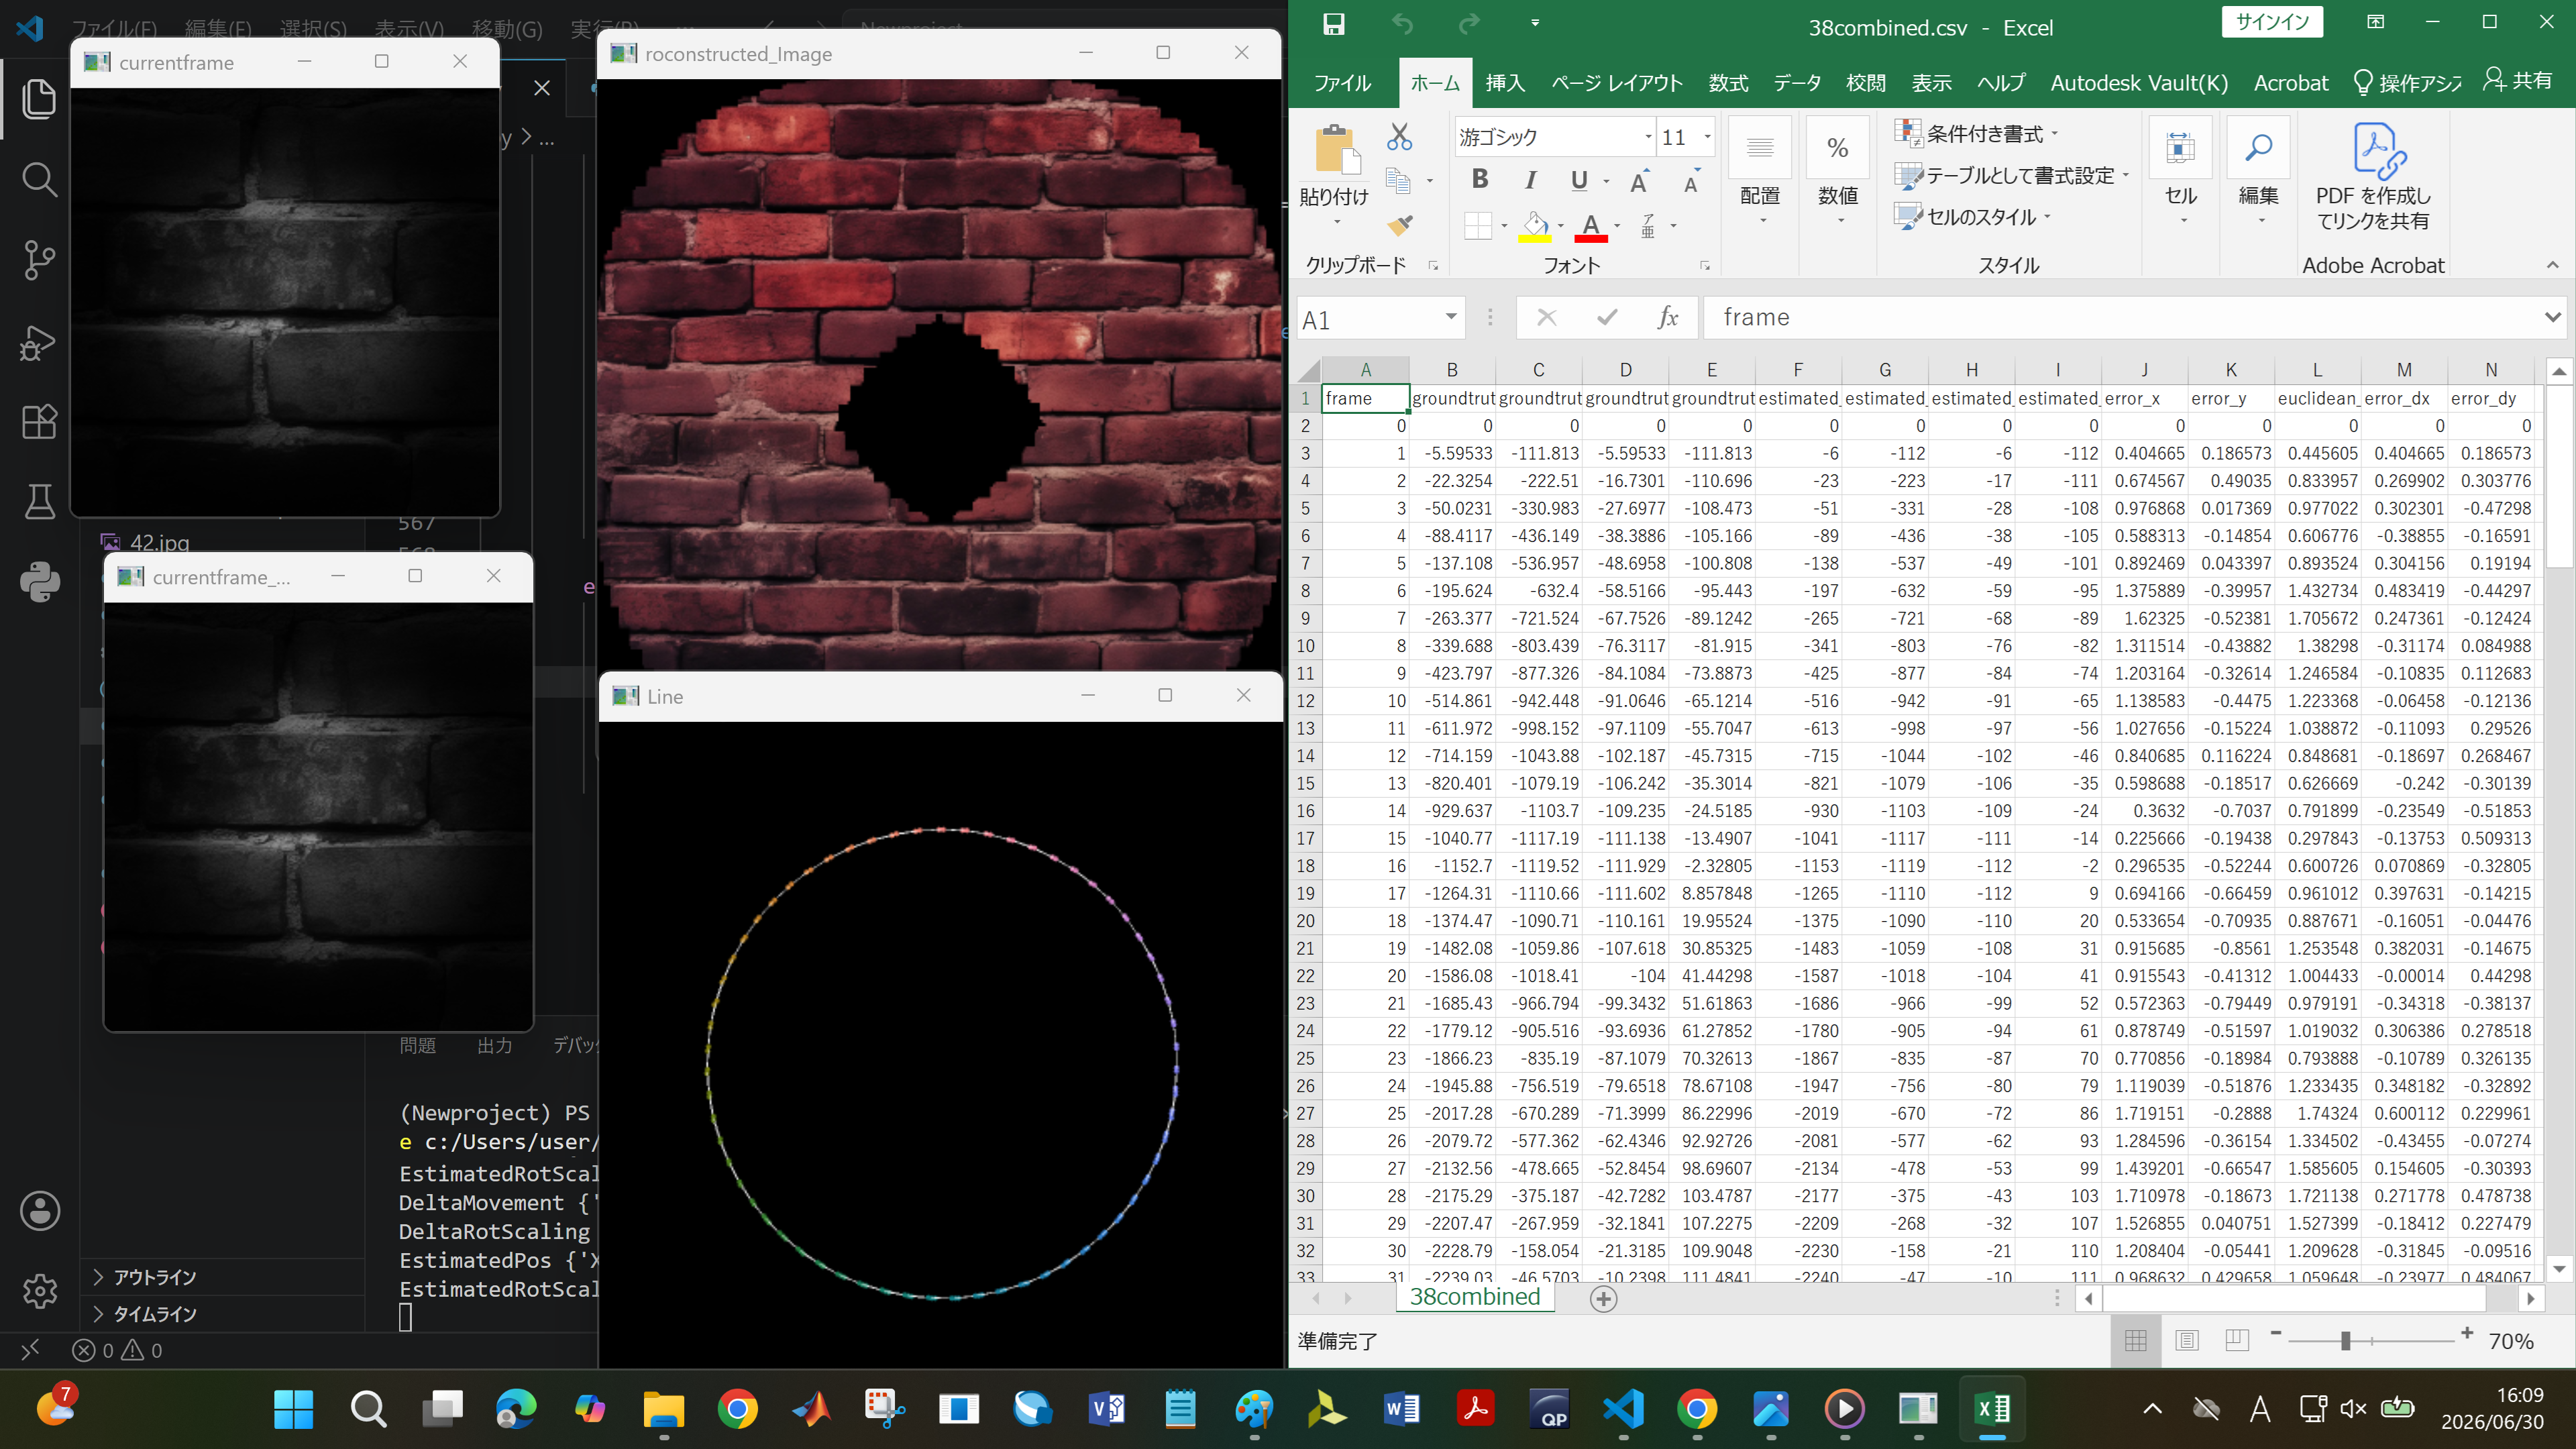
\includegraphics[width=\linewidth]{figures/誤差比較.png}
    \caption{誤差比較}
    \label{fig:誤差比較}
\end{figure}

\section{まとめ}
今週は誤差比較のための機能を実装した。

\section{来週やること}
\begin{enumerate}
    \item 画像フィルタの実装
    \item 処理時間の計測機能の実装
    \item ステップサイズに基づいたフレームの間引き処理
\end{enumerate}


\end{document}


